\section{数据分析与可视化}
\par{本报告使用可视化库为pyecharts,能够在web端实现数据交互查看,最终html文件位于ananlyze目录下,预览动态交互可运行vi\_merged.html可查看,以下部分仅展示静态图片。}

\subsection{逐年发微热力图}
统计分析每年中月日发微博频率,主要代码如下。
\begin{python}
    df = pd.read_csv('cleaned_text.csv', parse_dates=['created_at'])
    date_counts = df['created_at'].dt.date.value_counts()
    cal_result = [(date, count) for date, count in date_counts.items()]
    page = Page(page_title='共青团中央微博分析', layout=Page.DraggablePageLayout)
    for year in range(2019, 2024):
        calendar = (
            Calendar()
            .add("",
                 cal_result,
                 calendar_opts=opts.CalendarOpts(range_=str(year)),
                 daylabel_opts=opts.CalendarDayLabelOpts(name_map="cn"),
                 monthlabel_opts=opts.CalendarMonthLabelOpts(name_map="cn"),
                 )
            .set_global_opts(
                title_opts=opts.TitleOpts(title=f"{year} 年每天发微频率"),
                visualmap_opts=opts.VisualMapOpts(
                    max_=55, min_=5, orient="horizontal", is_piecewise=True, pos_top="230px", pos_left="100px",
                ),
            )
        )
\end{python}
逐年可视化热力图如下。
\begin{figure}[H]
    \centering
    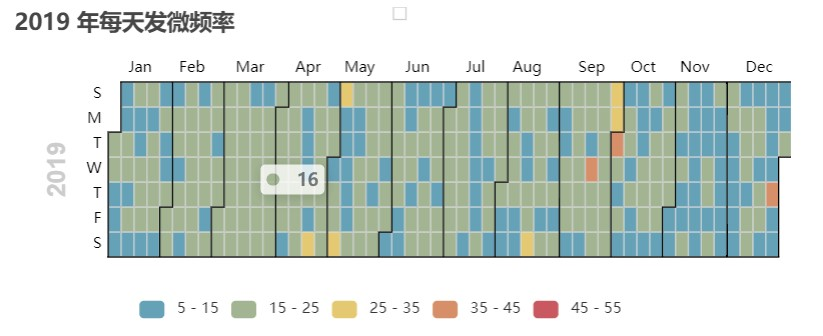
\includegraphics[width=12cm]{figure/2019.jpg}
    \caption{2019热力图} \label{fig:2019}
\end{figure}

\begin{figure}[H]
    \centering
    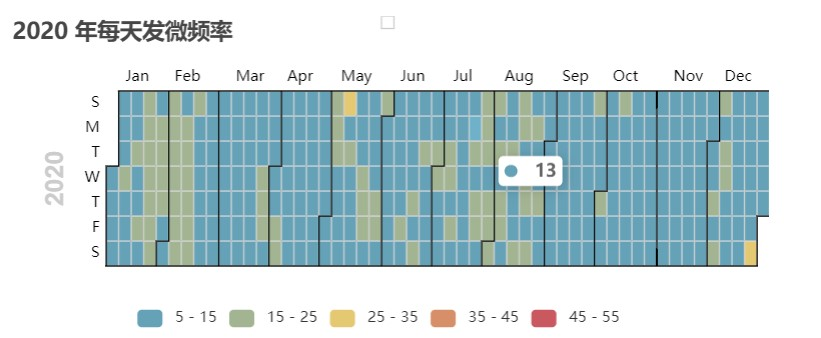
\includegraphics[width=12cm]{figure/2020.jpg}
    \caption{2020热力图} \label{fig:2020}
\end{figure}
\begin{figure}[H]
    \centering
    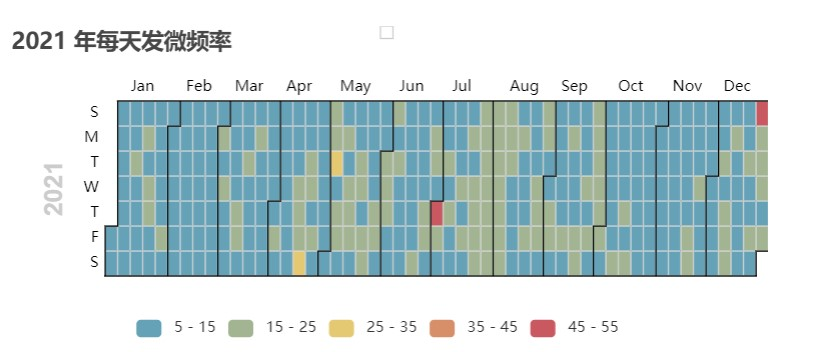
\includegraphics[width=12cm]{figure/2021.jpg}
    \caption{2021热力图} \label{fig:2021}
\end{figure}
\begin{figure}[H]
    \centering
    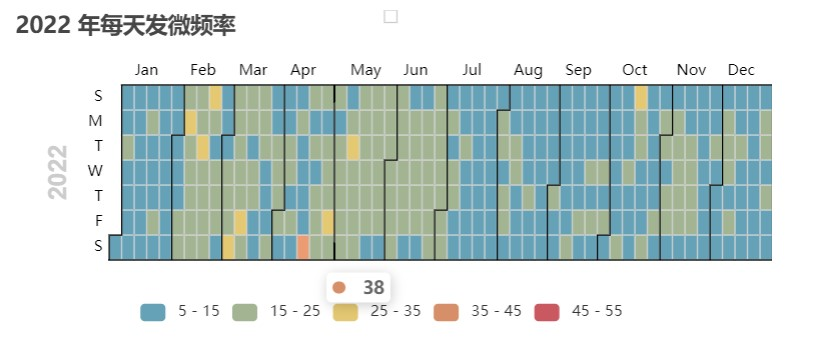
\includegraphics[width=12cm]{figure/2022.jpg}
    \caption{2022热力图} \label{fig:2022}
\end{figure}    
\begin{figure}[H]
    \centering
    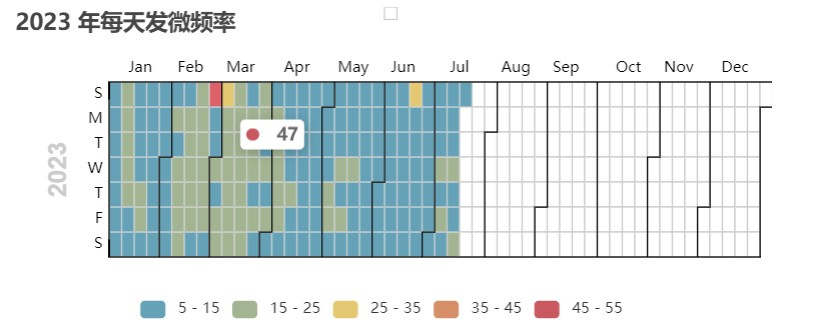
\includegraphics[width=12cm]{figure/2023.jpg}
    \caption{2023热力图} \label{fig:2023}
\end{figure}    

\subsection{发微时间统计}
使用pandas内置函数按照年、月、周、日、时分别统计共青团中央发微时间。
\begin{python}
    df = pd.read_csv('cleaned_text.csv', parse_dates=['created_at'])
    dateyear_counts = df['created_at'].dt.year.value_counts()
    datemonth_counts = df['created_at'].dt.month.value_counts()
    dateweek_counts = df['created_at'].dt.weekday.value_counts()
    dateday_counts = df['created_at'].dt.day.value_counts()
    datehour_counts = df['created_at'].dt.hour.value_counts()
\end{python}

\subsubsection{逐年统计}
利用pyecharts制作逐年统计可视化,结果如图\ref{fig:yearfre}所示。
\begin{python}
    c_year = (
        Bar()
        .add_xaxis([i[0] for i in resultyear])
        .add_yaxis("共青团中央", [i[1] for i in resultyear])
        .set_global_opts(
            title_opts=opts.TitleOpts(title="每年发微频率"),
            yaxis_opts=opts.AxisOpts(name="次数"),
            xaxis_opts=opts.AxisOpts(name="时间"),
        )

    )
\end{python}
\begin{figure}[H]
    \centering
    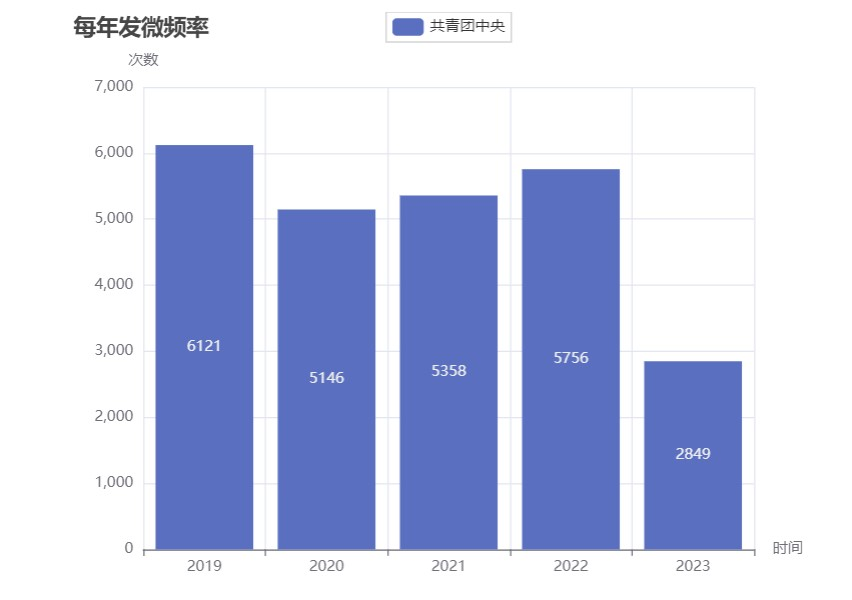
\includegraphics[width=12cm]{figure/yearfre.jpg}
    \caption{逐年统计} \label{fig:yearfre}
\end{figure} 
\subsubsection{每年逐月统计}
逐月统计可视化。
\begin{python}
    c_month = (
        Bar()
        .add_xaxis(Faker.months)
        .add_yaxis("共青团中央", [i[1] for i in resultmonth])
        .set_global_opts(
            title_opts=opts.TitleOpts(title="每月发微频率"),
            yaxis_opts=opts.AxisOpts(name="次数"),
            xaxis_opts=opts.AxisOpts(name="时间"),
        )

    )
\end{python}
\begin{figure}[H]
    \centering
    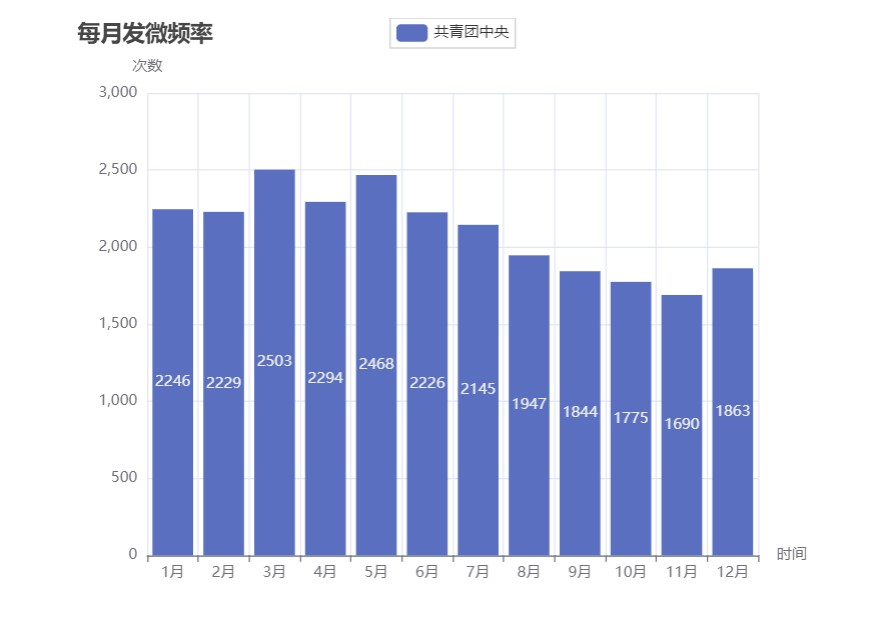
\includegraphics[width=12cm]{figure/monthfre.jpg}
    \caption{逐月统计} \label{fig:monthfre}
\end{figure} 
\subsubsection{每月逐天统计}
本小节后续部分与上述实现过程相似,不再赘述,仅展示最终可视化结果。
\begin{figure}[H]
    \centering
    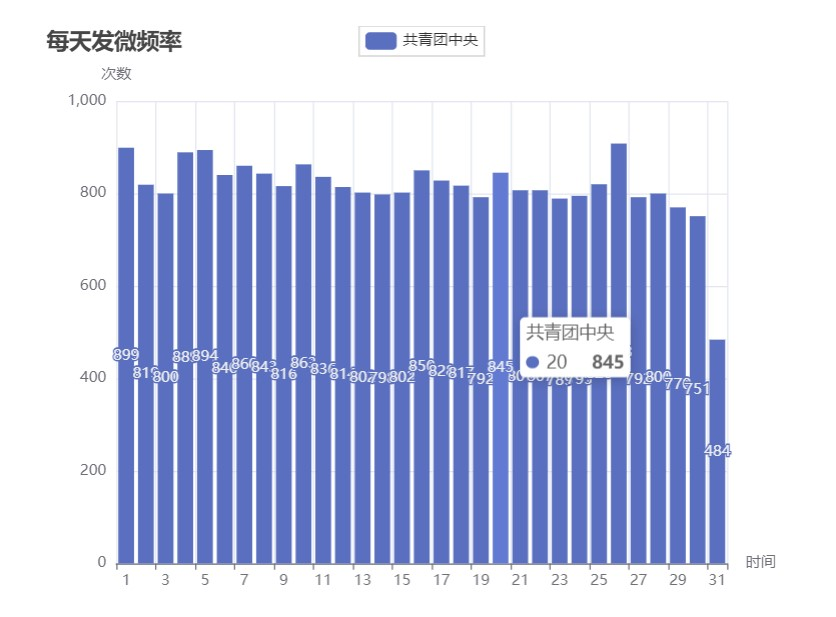
\includegraphics[width=12cm]{figure/dayfre.jpg}
    \caption{逐天统计} \label{fig:dayfre}
\end{figure} 
\subsubsection{每周逐天统计}
\begin{figure}[H]
    \centering
    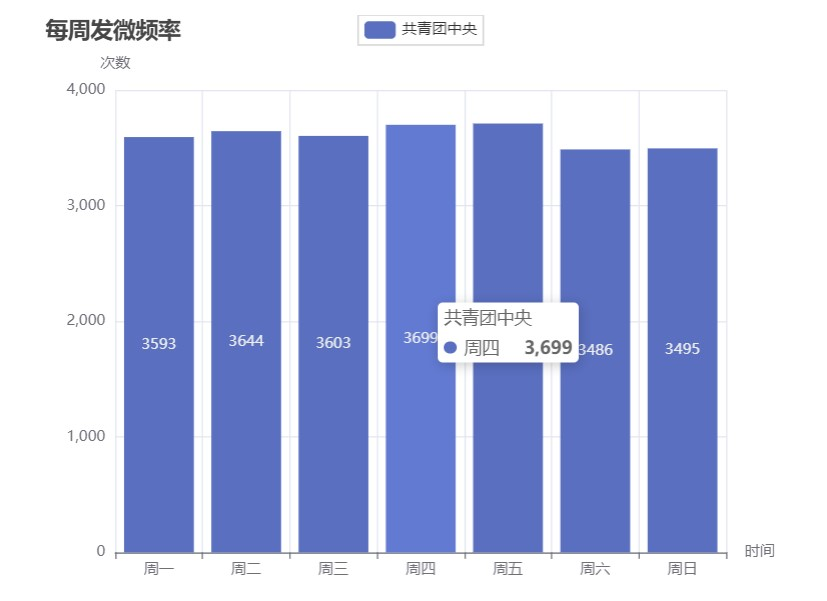
\includegraphics[width=12cm]{figure/weekdayfre.jpg}
    \caption{逐周统计} \label{fig:weekdayfre}
\end{figure} 
\subsubsection{每天逐时统计}
\begin{figure}[H]
    \centering
    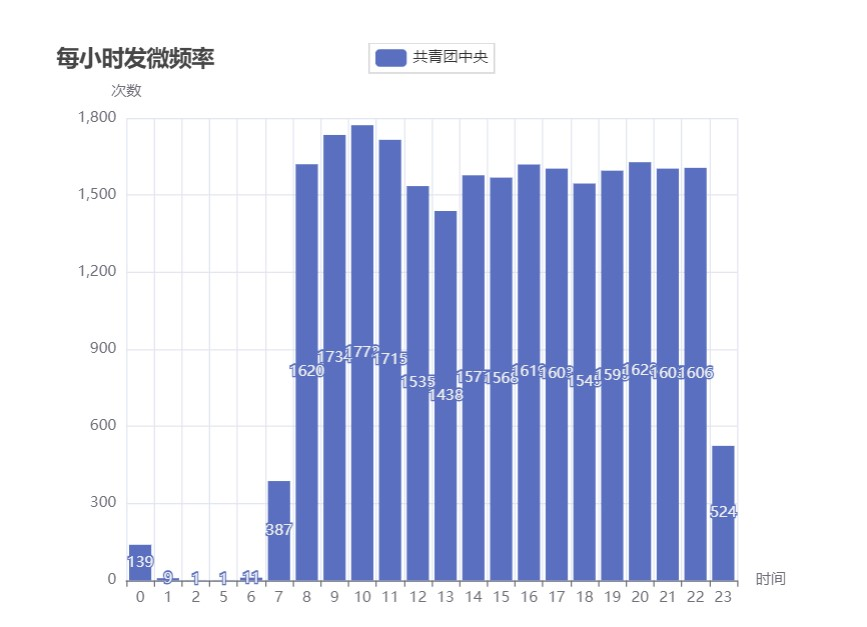
\includegraphics[width=12cm]{figure/hourfre.jpg}
    \caption{逐时统计} \label{fig:hourfre}
\end{figure} 
\subsection{周时热力统计}
\par{使用pandas的groupby多列分组先按照hour来分组。每组内,再按weekday来分组,并统计每个周时数量返回。}
\begin{python}
def to_weekhour(file, file_colm):
    df = pd.read_csv(file)
    df[file_colm] = pd.to_datetime(df[file_colm])
    hour_week_counts = df.groupby([df[file_colm].dt.hour, df[file_colm].dt.weekday])[file_colm].count()
    result = [[hour, week, count] for (hour, week), count in hour_week_counts.items()]
    result.sort(key=lambda x: x[0]) #按照第一个排序
    return result
\end{python}
\par{调用to\_weekhour函数将分类统计结果传回pyecharts进行可视化绘图,核心代码如下。}
\begin{python}
    c_heatmap = (
        HeatMap()
        .add_xaxis(Faker.clock)
        .add_yaxis(
            "发微次数", Faker.week, to_weekhour('cleaned_text.csv', 'created_at'),
            label_opts=opts.LabelOpts(position="middle")
        )
        .set_global_opts(
            title_opts=opts.TitleOpts(title="共青团中央发微周时热力图"),
            visualmap_opts=opts.VisualMapOpts(),
        )
    )
\end{python}
最终可视化效果如图\ref{fig:weekdayhour}
\begin{figure}[H]
    \begin{center}
    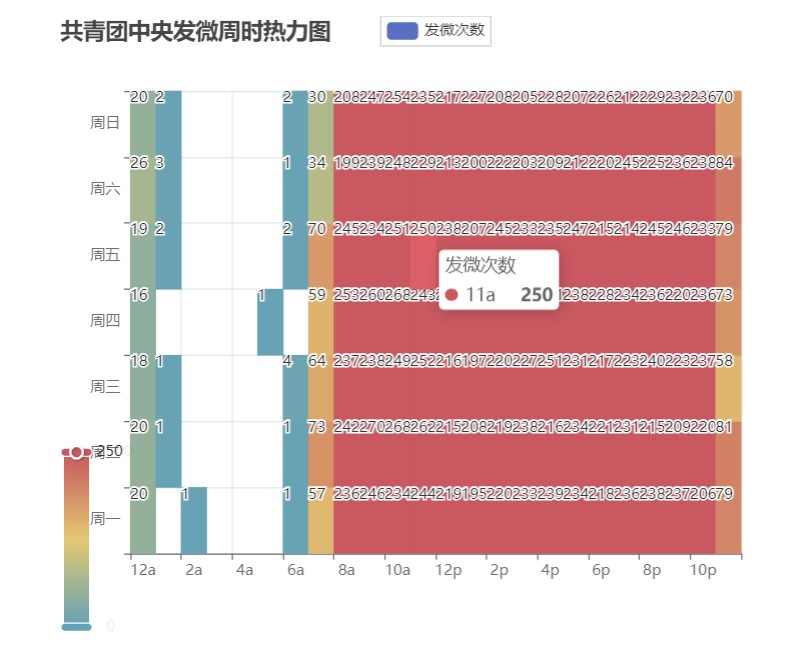
\includegraphics[width=14cm]{figure/weekday_hour.jpg}
    \caption{周时热力图}  \label{fig:weekdayhour}
    \end{center}
\end{figure}

\subsection{高频词统计}
定义函数统计词频,添加自定义词典和停用词词典,使用jieba库进行分词,jieba分词工具有三种主要分词模式,本报告选取\textbf{HMM}模式。
\begin{python}
def count_word_frequency(csv_file_path, column_name):
    df = pd.read_csv(csv_file_path)
    df[column_name].fillna('', inplace=True)
    content = df[column_name]
    merged_content = ' '.join(content)
    pattern = re.compile(u'\t|\n|\.|-|:|;|\)|\(|\?|"')
    string_data = re.sub(pattern, '', merged_content)
    jieba.suggest_freq('共青团', True)
    jieba.load_userdict('user_words.txt')
    seg_list_exact = jieba.cut(string_data, cut_all=False, HMM=True)  # 分词模式
    object_list = []
    # 去除停用词
    with open('stop_words.txt', 'r', encoding='UTF-8') as meaninglessFile:
        stopwords = set(meaninglessFile.read().split('\n'))
    stopwords.add(' ')
    for word in seg_list_exact:
        if word not in stopwords:
            object_list.append(word)
    word_counts = collections.Counter(object_list)
    for word in list(word_counts.keys()):
        if len(word) == 1:
            del word_counts[word]
    word_counts_top = word_counts.most_common(300)
    return word_counts_top
\end{python}
\par{使用pyecharts制作词云可视化,此外本报告也采用了自定义功能更强大的wordcloud库结合matplot等库制作了共青团中央微博内容词云可视化,相关结果为摘要页微博图标背景的词云可视化图片。}

\begin{python}
    c_wordcloud = (
        WordCloud()
        .add(
            "",
            count_word_frequency('cleaned_text.csv', 'content'),
            word_size_range=[20, 100],
            textstyle_opts=opts.TextStyleOpts(font_family="cursive"),
        )
        .set_global_opts(title_opts=opts.TitleOpts(title="top200词云"))
    )
\end{python}
使用pyecharts实现的可视化效果如图所示,能够实现在网页端点击悬停等交互。
\begin{figure}[H]
    \centering
    
\includegraphics[width=12cm]{figure/wordcloud_pyecharts.jpg}
    \caption{词频统计词云} \label{fig:wordcloud}
\end{figure} 

\subsection{LDA主题分析}
\par{首先对文本内容进行分词,分词程序位于analyze/LDA/cutword.py,具体实现与词云处一致调用jieba库。分词后,基于已分词文档使用gensim库进行LDA主题分析,并使用pyLDAvis进行可视化展示。思路阐述参考下列代码注释}\
\begin{python}
import pyLDAvis.gensim_models
from gensim.corpora.dictionary import Dictionary
from gensim.models.ldamodel import LdaModel
from gensim import corpora, models

if __name__ == '__main__':
    words_ls = []
    with open('outdemowei.txt', 'r', encoding='UTF-8') as f:
        data = f.readlines()
        for line in data:
            words_ls.append(line.split(' '))
    f.close()
    # 构造词典,将每个唯一的词语映射到一个唯一的整数ID
    dictionary = corpora.Dictionary(words_ls)
    # 基于词典,使【词】→【稀疏向量】,并将向量放入列表,形成【稀疏向量集】(即语料库)
    corpus = [dictionary.doc2bow(words) for words in words_ls]
    # tf-idf编码
    tfidf = models.TfidfModel(corpus)
    # 将语料库转换为tf-idf编码形式
    corpus_tf = tfidf[corpus]
    # lda模型,num_topics设置主题的个数
    lda = LdaModel(corpus=corpus_tf, id2word=dictionary, num_topics=4, random_state=100, iterations=50)

    for topic in lda.print_topics(num_words=10):
        print(topic)
    # 用pyLDAvis可视化
    plot = pyLDAvis.gensim_models.prepare(lda, corpus_tf, dictionary)
    pyLDAvis.save_html(plot, 'ldaweibo.html')

\end{python}
通过LDAModel抽取4个主题后,最终可视化效果如图\ref{fig:lda}所示,html可视化源文件位于analyze/LDA/ldaweibo.html。
\begin{figure}[H]
    \centering
    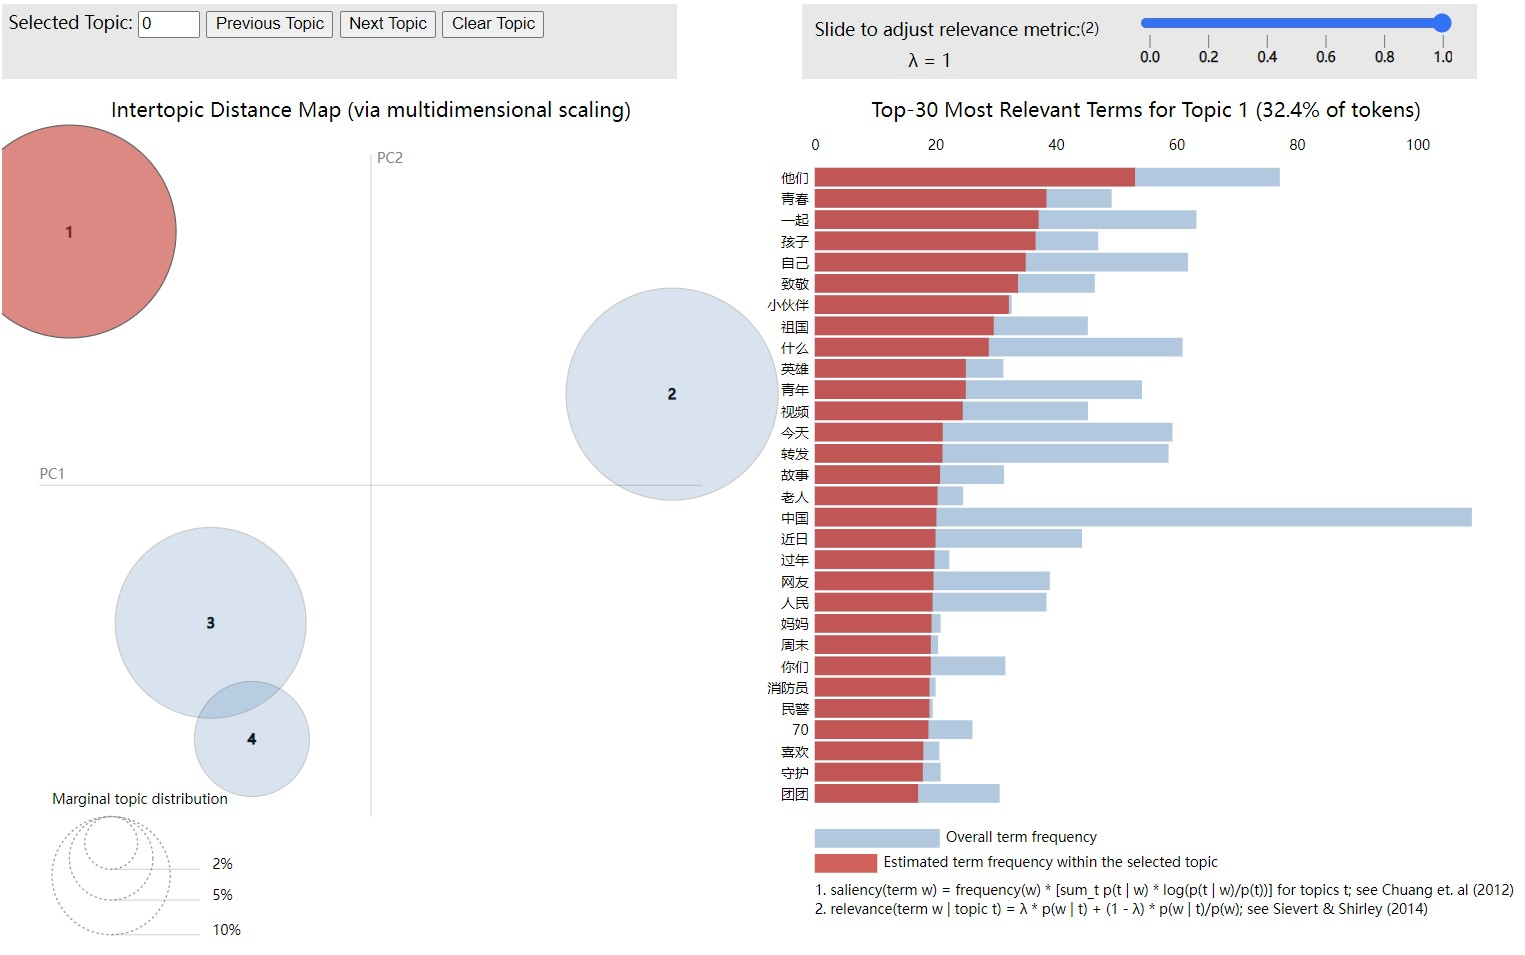
\includegraphics[width=12cm]{figure/lda.jpg}
    \caption{LDA分析结果} \label{fig:lda}
\end{figure} 
